\documentclass[12pt,letterpaper]{article}

\usepackage{caption} % for the figure captions
\usepackage[osf]{mathpazo} % a nicer font
% this is a package for the citation formats: found this formulation sorted natbib errors when changing packages
%from http://tex.stackexchange.com/questions/54480/package-natbib-error-bibliography-not-compatible-with-author-year-citations
\usepackage[square,sort,comma,numbers]{natbib} 
\usepackage{amsmath} % package for equations
\usepackage{url} % package for urls
\usepackage{hyperref} % for hyperlinks
\hypersetup{
     colorlinks   = true,
     citecolor    = gray
}
\usepackage{graphicx} % for the figures
\usepackage{pdfpages}

\hypersetup{linkcolor=blue}

\pagenumbering{arabic} % stating the page number type

\graphicspath{ {Images/} }

%Title page
%Itinerary
%Localities
%Kit list
%Contact details
%Where staying: all deets

\begin{document}

\title{Scotland Field Trip Manual}
\maketitle

\pagebreak

\tableofcontents


\pagebreak

%------------------------------
%Itinerary
%------------------------------

\section{Itinerary}

\begin{table}[!htpb]
\centering
\begin{tabular}{l l l}
	\textbf{Dates} & \textbf{Activity} & \textbf{People} \\
	\hline
	15th June & Richard arrives in Edinburgh and sorts initial food shopping\\
	16th June & Everyone joins Richard in Edinburgh over the course of the day\\
	17th June & Drive from Edinburgh to Monikie\\
	18th June & Work Tillywhandland - Bob Davidson may join\\
	19th June & Work Tillywhandland - Bob Davidson may join\\
	20th June & Work Tillywhandland - Bob Davidson may join\\
	21st June & Work Tillywhandland - Bob Davidson may join\\
	22nd June & Drive from Monikie to North Kessock \\
	23rd June & Work Cromarty and Eathie \\
	24th June & Drive from North Kessock to Thurso.  Possibly work Thurso \\
	25th June & Work Achanarras \\
	26th June & Drive from Thurso to Stromness \\
	27th June & Work Cruaday Quarry - joined by John Brown \\
	28th June & Work Cruaday Quarry \\
	29th June & Fun day of Orcadian fun \\
	30th June & Drive back from Stromness to Inverness \\
	1st July & Fly back to London \\

\end{tabular} \\
\end{table}

\pagebreak

%------------------------------
%Localities
%------------------------------

\section{Locality information}

\indent All of the localities we're going to are part of the Old Red Sandstone, famous for its Devonian fishes.  I've written a brief introduction to each one below: this is based on Dineley and Metcalf's `Fossil Fishes of Great Britain' help from Mike Newman, and googling.  The book is now out of print, but you can find individual chapters by googling site names. \newline

At the majority of the sites we will be looking for material for Martin's teaching collection, but at the first (Tillywhandland), we will hopefully also find material pertinent to my PhD project. \newline

Many of the sites are also SSSIs (sites of special scientific interest).  This means that it is illegal to take fossils out of the cliff, and it's probably best to keep any geological hammers etc out of plain site so you don't look like you're about to. Otherwise we're covered by (and ought to follow) the Scottish Fossil Code - this provides a set of guidelines and rules for collecting fossils in Scotland and is worth a skim, but essentially it amounts to don't be a dickhead.  \newline

The Scottish Fossil Code can be found here: \url{http://goo.gl/9KrOS7}

\begin{figure}[h!]
\caption{Locations of sites}
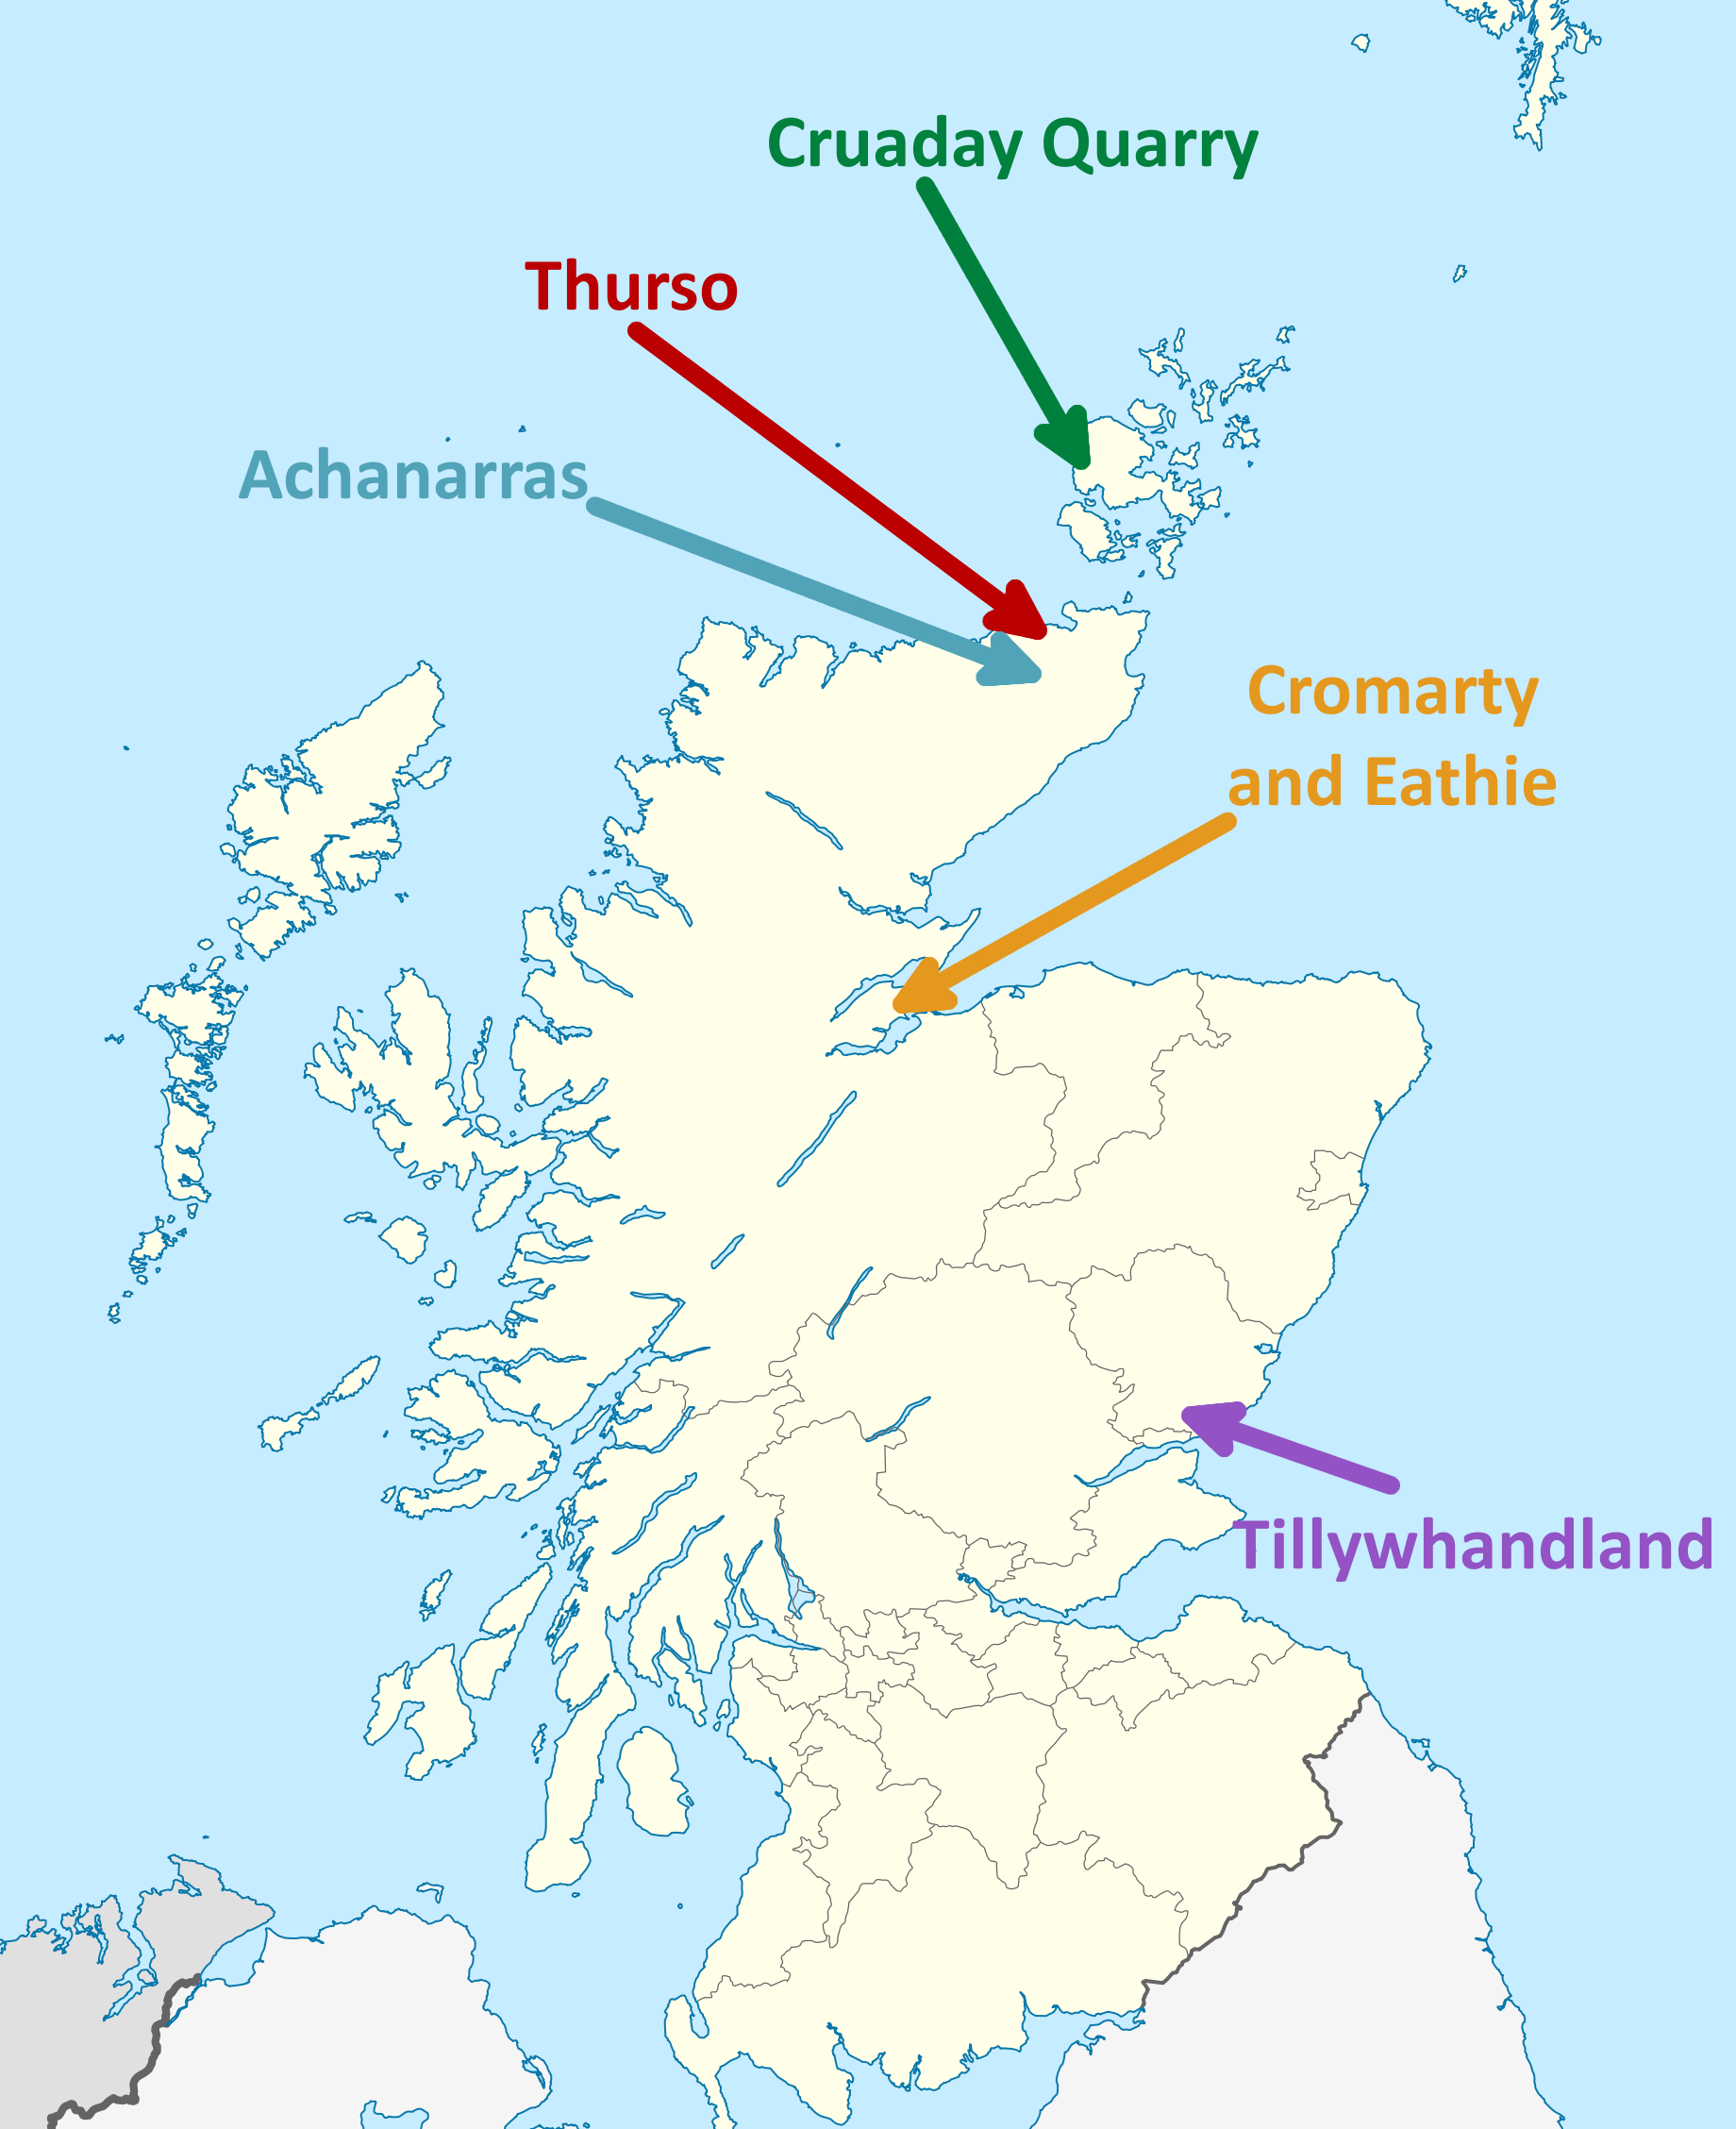
\includegraphics[scale=0.2]{Scotland_sites}
\centering
\end{figure}

\pagebreak

\subsection{Tillywhandland}

Tillywhandland is thought to be the source of many Scottish Old Red Sandstone fossils from ``Turin Hill''; 19th century sandstone quarrying at this site revealed a number of fossils including acanthodians, osteostracans, and eurypterids which were described by Powrie and others.  The fish bearing rock is a laminite, comprising clastic, organic, and carbonate layers.  This is interpreted as having been laid down in a shallow seasonal lake, Lake Forfar, in the Early Devonian.  The fishy denizens of this lake (and/or surrounding rivers) were preserved in the anoxic sediment at its bottom.\newline

\begin{figure}[h!]
\caption{A reconstruction of Lake Forfar from Trewin and Davidson (1996)}
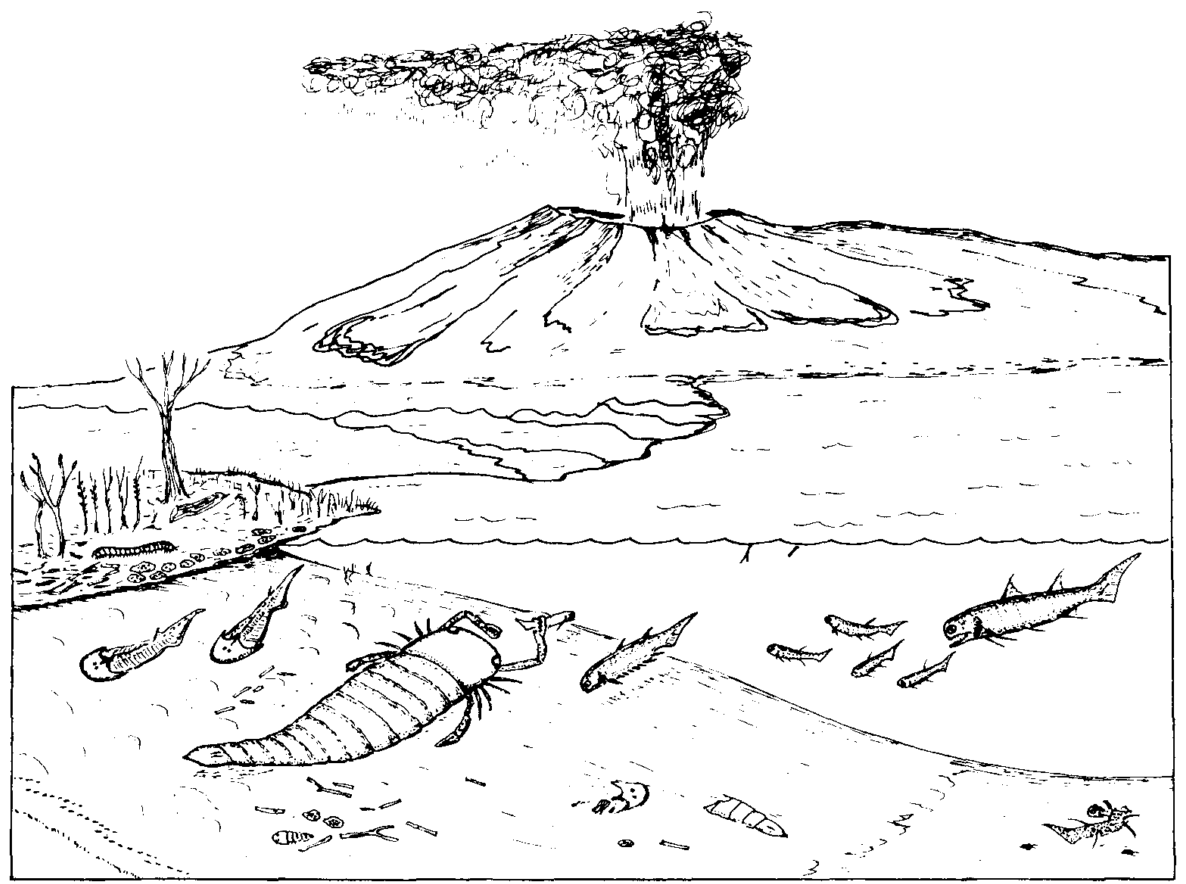
\includegraphics[scale=0.6]{Lake_Forfar}
\centering
\end{figure}

Fishy fossils at Tillywhandland are found only in one fish bearing bed, and are fairly few and far between: if you want to get your eye in for what these look like, we've got some in the lab. Fishes include the osteostracan \textit{Cephalaspis}, and the acanthodians \textit{Climatius}, \textit{Ischnacanthus}, \textit{Euthacanthus}, \textit{Vernicomacanthus}, \textit{Mesacanthus}, and possibly \textit{Brachyacanthus} and \textit{Uraniacanthus}: with modern acid preparation techniques these fishes are comparable in preservation to those from the much-vaunted Man on the Hill (MOTH) locality in Canada  We're (or at least I am) particularly interested in the acanthodian \textit{Vernicomacanthus uncinatus}: I'm redescribing it as part of my PhD work and it displays an intiguing mixture of ``acanthodian'' and ``chondrichthyan'' characters.  We may also find the eurypterid \textit{Pterygotus}, millipedes, arthropod trackways, plant material, and coprolites.  \newline

\begin{figure}[h!]
\caption{The holotype of \textit{V. uncinatus} from ``Turin Hill''}
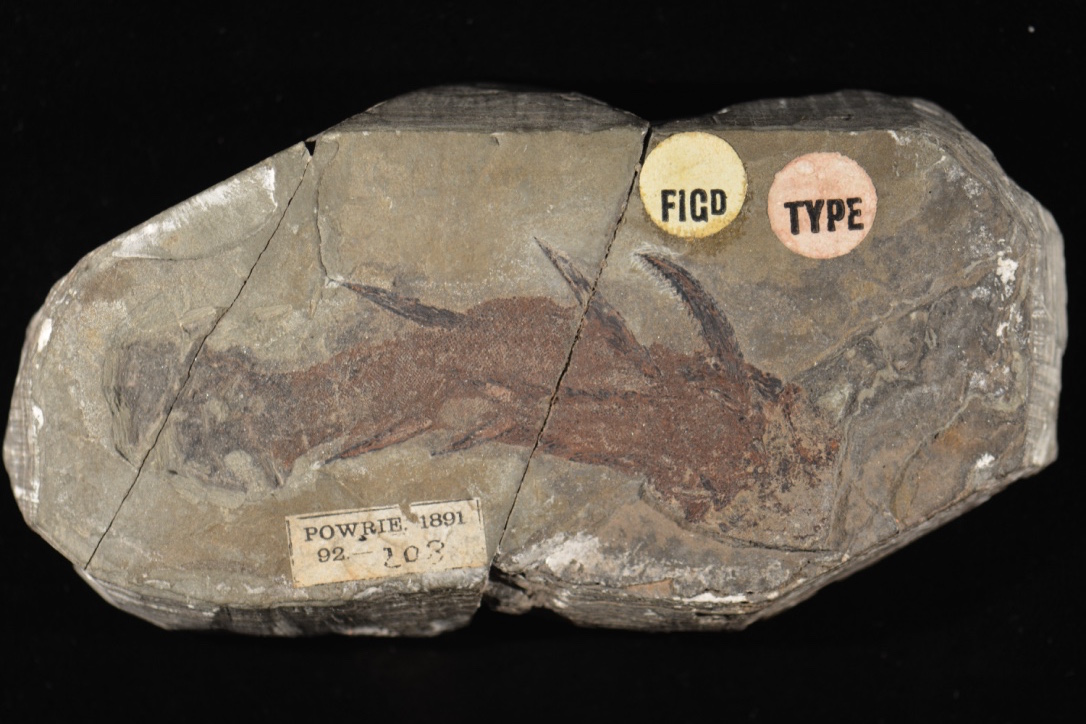
\includegraphics[scale=0.35]{Vernicomacanthus}
\centering
\end{figure}

Bob Davidson, who wrote a description of Tillywhandland and who has a lot of experience working there, will hopefully be joining us for a day.  The land is privately owned by a Mr Middleton, who John Armstrong (another guy who works Tillywhandland regularly) has kindly contacted to let him know we're coming.\newline


\subsection{Cromarty and Eathie}

Cromarty and Eathie (as well as all of the rest of our sites) are from the Orcadian basin, a sedimentary basin laid down by Lake Orcadie in the Middle Devonian.  These sites are on the coast of the Black Isle, a peninsula (rather than an island) that juts out of the east coast of Scotland between the Cromarty, Beauly, and Moray Firths.  Cromarty was the birthplace of the famous Scottish geologist Hugh Miller (1802-1856), and according to something I read on the internet the footpath down to the rocks at Eathie was built by him \textsuperscript{[citation needed]}.  

These sites also have a Jurassic exposure: the Devonian fishes are all in concretions along the foreshore.

\subsection{Achanarras}

Achanarras is an extremely rich site from the Southwestern part of Lake Orcadie.  It's probably most famous for \textit{Palaeospondylous}, the enigmatic early vertebrate large quantities of which take up space in museum drawers all across the UK.  Fishes are to be found in limestone laminites in several horizons: these include acanthodians \textit{Mesacanthus}, \textit{Cheiracanthus} and \textit{Diplacanthus}, placoderms \textit{Coccosteus}, \textit{Homosteus},\textit{Pterichthyodes}, and \textit{Rhamphodopsis}, and osteichthyans \textit{Cheirolepis}, \textit{Glyptolepis}, \textit{Osteolepis}, and \textit{Dipterus}.  These can be found by splitting the limestone flags.

The land is public, but is an SSSI.  Mike Newman tells me the spoil tips have recently been turned by a JCB, so it may be productive. Sometimes the quarry is flooded, if we don't get anywhere we can go to the next site, Thurso.

\subsection{Thurso}

The beach in Thurso where we are staying provides another exposure of the Orcadian basin and is similar to Achanarras: if we get a chance on one of the driving days or if Achanarras is unproductive, we could check it out.  There are no restrictions.

\begin{figure}[h!]
\caption{Bring your Geiger counters}
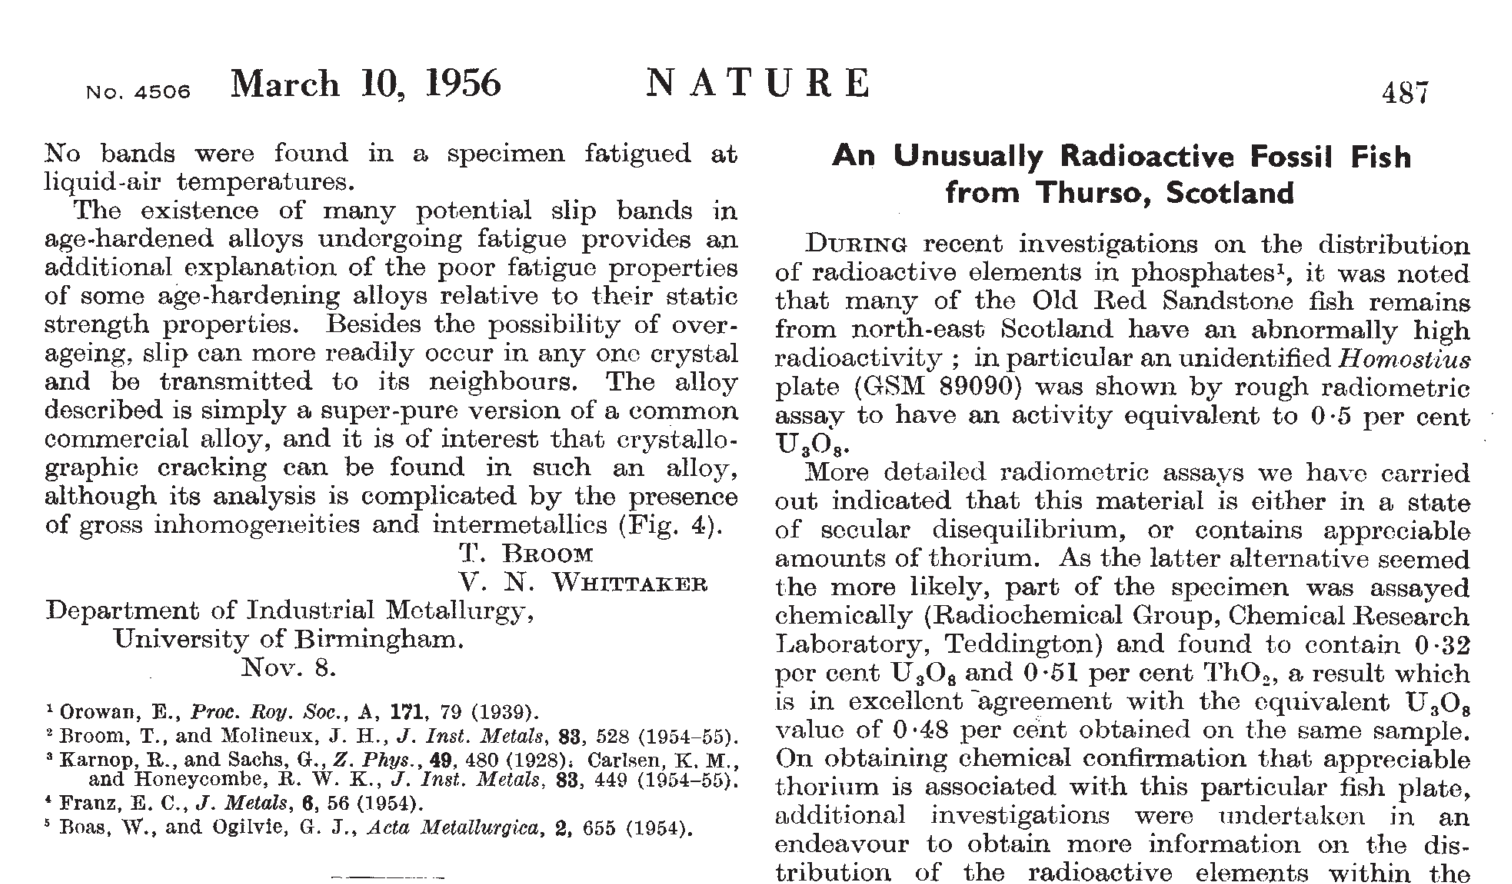
\includegraphics[scale=0.5]{Radioactive_fish}
\centering
\end{figure}

\subsection{Cruaday Quarry}

Cruaday Quarry is the most high-profile exposure of the Sandwick fish beds in the Orkneys, located near the lewdly-named village of Twatt on the Western side of the Mainland.  Fishes are preserved in a fish layer formed from dark grey siltstones. It has a similar collection of fishes to other Lake Orcadie sites, including acanthodians \textit{Diplacanthus}, \textit{Rhadinacanthus}, \textit{Mesacanthus}, and \textit{Cheiracanthus}, placoderms \textit{Pterichthyodes}, \textit{Coccosteus}, and \textit{Homosteus}, and osteichthyans \textit{Osteolepis}, \textit{Cheirolepis}, \textit{Gyroptychius}, and \textit{Dipterus}.

If we have time in the afternoon after the ferry there is a museum of Orkney Fossils on the island of Burray: we could go there to get our eye in for what we're looking for, dependent on tiredness/time.

The quarry is in active use (owned by Orkney Aggregates), but the main fish bed part is controlled by John Flett Brown, the chairman of the fossil museum on Burray: John will be coming with us on one of the days to show us around the site.  This site is also an SSSI.

\subsection{The Highland Park Distillery}

On our final day in the Orkneys we will be visiting perhaps the most important locality of all: the Highland Park distillery in Kirkwall, the ``capital'' of the Orkneys.  Currently the plan is to go to Skara Brae in the morning, a stone-built Neolithic village that is part of a UNESCO world heritage site that covers several sites in the Orkneys.  We will then drive to Kirkwall: on the way we will also see the Ring of Brodgar, a stone henge that is also part of the world heritage site, as well as the remains of the fleet scuppered by the German Navy in the Scapa Flow at the end of the First World War. I've booked us onto an hour-long tour at the distillery at 2pm.  After that we can do whatever we want in Kirkwall.

Obviously these activities won't be covered by the lab, so bring some money: the distillery tour costs £7.50 a head.




%------------------------------
%Kitlist
%------------------------------

\pagebreak
\section{Kit list}

I've put a list of things you'll need below: please try and pack reasonably lightly as there won't be enormous amounts of room in the car.
\linebreak
\begin{itemize}
  \item Clothing - ensure you bring warm things.
  \item Raincoat and ideally waterproof trousers. Scotland is wet.
  \item Some kind of sun protection: hat and cream.
  \item Walking boots: something with ankle support.  Thomas, your shitkickers will probably do.
  \item A towel and washing things- not sure we'll need the towel, but best to be safe - I'll check
  \item A hand lens
  \item Geological hammer: not strictly necessary, and we may not be able to use them at some localities, but if you've got one bring it in case
\linebreak
\linebreak
\linebreak
  \item We will bring lab chisels, hard hats, and a crackhammer, so no need for them
  \item No need for a sleeping bag: all the places provide begging (?)

\end{itemize}

\pagebreak


%------------------------------
%The trip
%------------------------------
\section{The trip}


\pagebreak
%------------------------------
%Accommodation details
%------------------------------
\section{Accommodation details}

\subsection{Edinburgh: nights of 15th/16th June}

The \textbf{Princes Street Travelodge} is just off Princes Street, the road that separates Edinburgh Old Town from New Town. It's 2 minutes walk from Edinburgh Waverley train station.

\begin{figure}[h!]
\caption{Directions from the station to the Travelodge}
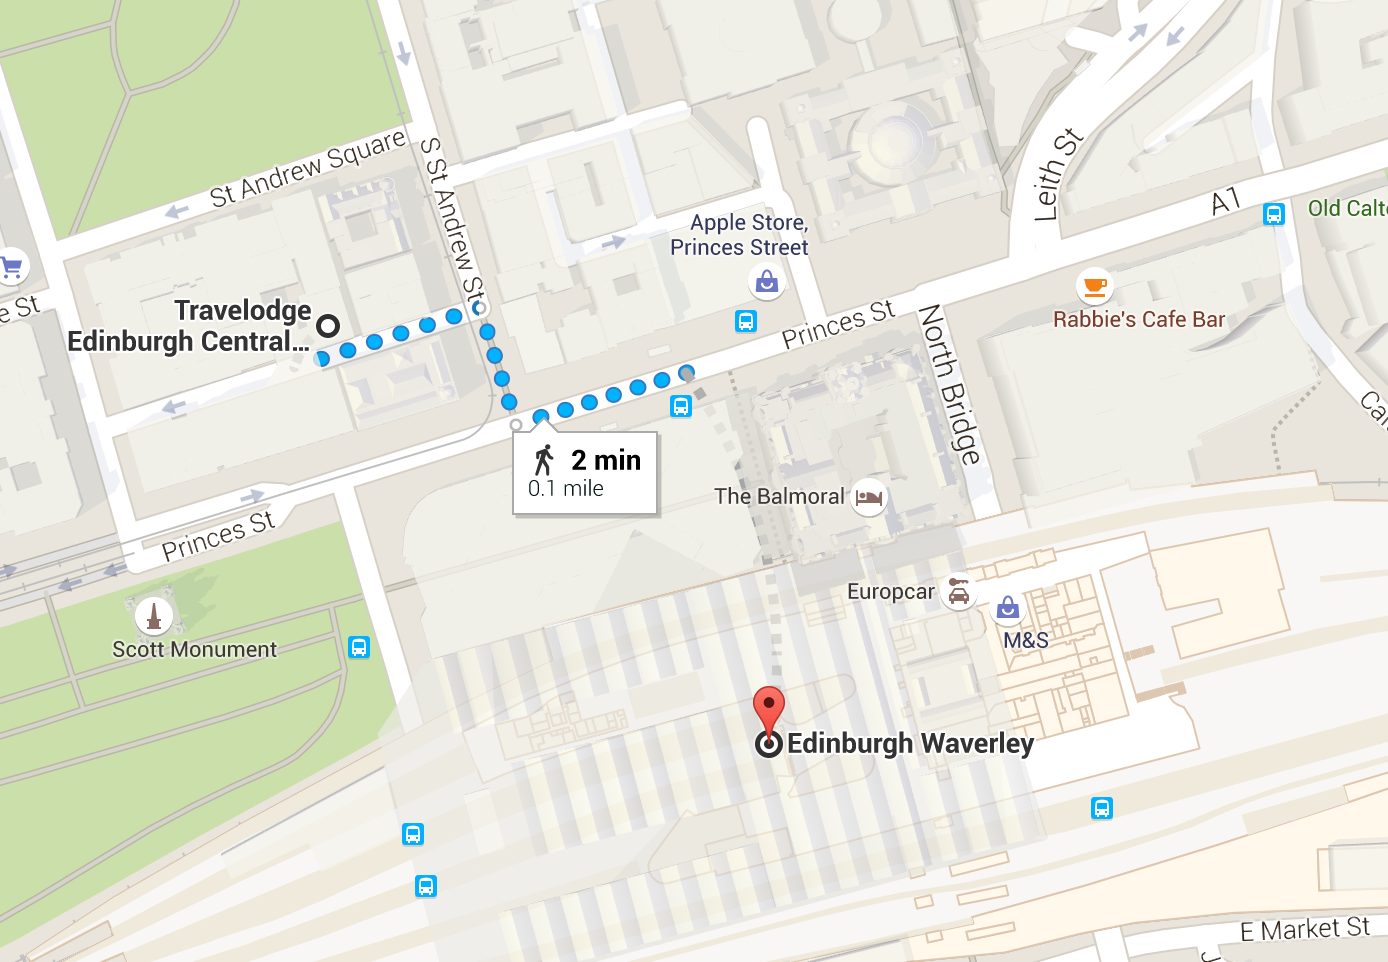
\includegraphics[scale=0.6]{Ed_direc}
\centering
\end{figure}

\textbf{Address:} Meuse Lane, off Princes Street, Edinburgh EH2 2BY, United Kingdom, EH2 2BY
\textbf{Telephone number:} 08715 591855

\begin{figure}[h!]
\caption{This is the picture that Google Maps associates with the Travelodge. A charming place indeed.}
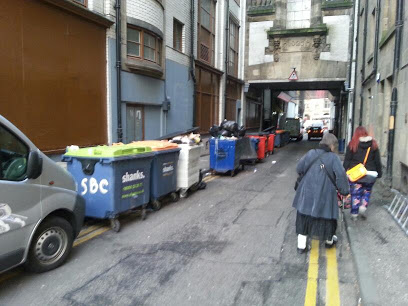
\includegraphics[scale=1]{Travelodge}
\centering
\end{figure}

\subsection{Monickie: nights of 17th-21st June}

For Tillywhandland we will be staying in the Monument Cottage in Monickie.  It has free private parking and wifi: we'll have to cook ourselves.

Monument Cottage, 
Monikie, 
Nr Broughty Ferry, 
Dundee,, Monikie, 
DD5 3QN

Contact no: 01382 370633

\subsection{North Kessock: nights of 22nd/23rd}

For Cromarty and Eathie we will be staying in an Airbnb in North Kessock, near Inverness.

The Anchor and Chain Coulmore, 
North Kessock, 
Ross Shire 
IV1 3XB

Contact no: 07545 586849

\subsection{Thurso: nights of 24th/25th}

For Achanarras/Thurso we will be staying in Thurso at the Royal Hotel

Royal Hotel
Traill Street, 
Thurso, 
KW14 8EH

Contact no: 01847 893191

\subsection{Stromness: nights of 26th-29th}

For Stromness we will be staying in Orkney self catering Loretto cottage.

Loretto,
Hillside Road,
Stromness,
Orkney,
KW16 3HR

Contact no: 01856 771865


\subsection{Inverness: night of 30th}

On the final night in Inverness we will be staying at The Waverley Guest House.

The Waverley Guest House,
25 Union Street,
Inverness,
IV1 1QA

Contact no: 01463 716008



\pagebreak
%------------------------------
%Contact details
%------------------------------

\section{Contact details}

\begin{table}[!htpb]
\centering
\begin{tabular}{l l}
	\textbf{Name} & \textbf{Mobile}\\
	\hline

	Richard & 07513 420621 \\
	Martin & 07938 638459 \\
	Anna & 07716037619 \\
	Marco & 07513494235 \\
	Victoria & 07713944767 \\
	Thomas &  +353 877 021326 \\
	Bob Davidson & ????? ?????? \\
	Rob Sansom & ????? ??????? \\
	Emma Randle & ????? ?????? \\
	John Flett Brown & ????? ??????? \\


\end{tabular} \\
\end{table}

\pagebreak

%------------------------------
%Appendices
%------------------------------



\end{document}